\documentclass{beamer}
\usepackage[utf8]{inputenc}

\usetheme{Madrid}
\usecolortheme{default}
\usepackage{amsmath,amssymb,amsfonts,amsthm}
\usepackage{txfonts}
\usepackage{tkz-euclide}
\usepackage{listings}
\usepackage{adjustbox}
\usepackage{array}
\usepackage{tabularx}
\usepackage{gvv}
\usepackage{lmodern}
\usepackage{circuitikz}
\usepackage{tikz}
\usepackage{graphicx}
\usepackage{multicol}

\setbeamertemplate{page number in head/foot}[totalframenumber]

\usepackage{tcolorbox}
\tcbuselibrary{minted,breakable,xparse,skins}

\definecolor{bg}{gray}{0.95}
\DeclareTCBListing{mintedbox}{O{}m!O{}}{%
  breakable=true,
  listing engine=minted,
  listing only,
  minted language=#2,
  minted style=default,
  minted options={%
    linenos,
    gobble=0,
    breaklines=true,
    breakafter=,,
    fontsize=\small,
    numbersep=8pt,
    #1},
  boxsep=0pt,
  left skip=0pt,
  right skip=0pt,
  left=25pt,
  right=0pt,
  top=3pt,
  bottom=3pt,
  arc=5pt,
  leftrule=0pt,
  rightrule=0pt,
  bottomrule=2pt,
  toprule=2pt,
  colback=bg,
  colframe=orange!70,
  enhanced,
  overlay={%
    \begin{tcbclipinterior}
    \fill[orange!20!white] (frame.south west) rectangle ([xshift=20pt]frame.north west);
    \end{tcbclipinterior}},
  #3,
}
\lstset{
    language=C,
    basicstyle=\ttfamily\small,
    keywordstyle=\color{blue},
    stringstyle=\color{orange},
    commentstyle=\color{green!60!black},
    numbers=left,
    numberstyle=\tiny\color{gray},
    breaklines=true,
    showstringspaces=false,
}

\numberwithin{equation}{section}
\lstset{
  language=Python,
  basicstyle=\ttfamily\small,
  keywordstyle=\color{blue},
  stringstyle=\color{orange},
  numbers=left,
  numberstyle=\tiny\color{gray},
  breaklines=true,
  showstringspaces=false
}

\title{Problem 3.3.14.}
\author{Sarvesh Tamgade}

\date{\today} 
\begin{document}

\begin{frame}
\titlepage
\end{frame}

\section{Question}
\begin{frame}{Question}
\textbf{Question}:
 Construct a right triangle in which the sides, (other than the hypotenuse) are of length 6 cm and 8 cm.
\end{frame}

\section{Solution}
\begin{frame}[fragile]
    \frametitle{Solution}
Let the two perpendicular sides have lengths 6 cm and 8 cm respectively.

Assume vertices:
\[
\vec{A} = \myvec{0 \\ 0}, \quad
\vec{B} = \myvec{6 \\ 0}, \quad
\vec{C} = \myvec{6 \cos 90^\circ \\ 8 \sin 90^\circ} = \myvec{0 \\ 8}
\]



This forms a right angle at vertex \(B\).



\end{frame}
\section{Graph}
\begin{frame}
    \frametitle{Graph}
    \begin{figure}[htbp]
    \centering
    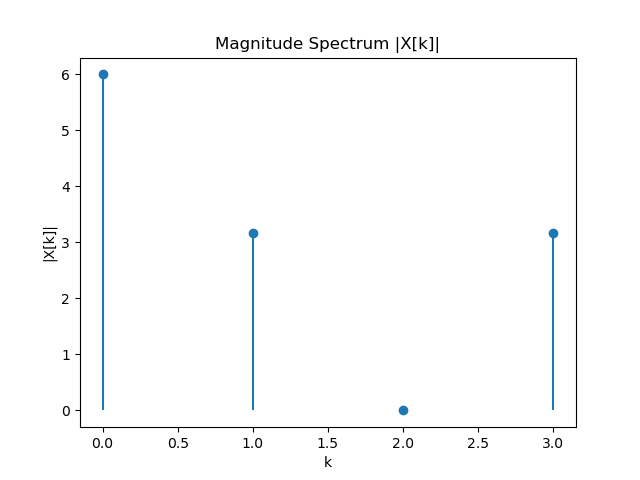
\includegraphics[width=0.65\linewidth]{FIG/fig1.png}
    \caption{Vector Representation}
    \label{fig:FIG/fig1.png}
\end{figure}
\end{frame}
\section{ C Code}
\begin{frame}[fragile]
\frametitle{C Code }
\begin{lstlisting}[language=C]
#include <stdio.h>
#include "trianglefun.h"

int main() {
    Point A, B, C;

    construct_right_triangle(&A, &B, &C);

    printf("Coordinates of triangle vertices:\n");
    printf("A: (%.2f, %.2f)\n", A.x, A.y);
    printf("B: (%.2f, %.2f)\n", B.x, B.y);
    // Print symbolic expression alongside evaluated coordinate for C
    printf("C: (6 * cos(90°) = %.2f, 8 * sin(90°) = %.2f)\n", C.x, C.y);

    return 0;
}


    
\end{lstlisting}
\end{frame}


\begin{frame}[fragile]
\frametitle{Python Code for Plotting}
\begin{lstlisting}[language=Python]
import matplotlib.pyplot as plt
import numpy as np

# Define vertices A, B, C
A = np.array([0, 0])
B = np.array([6, 0])
C = np.array([6 * np.cos(np.radians(90)), 8 * np.sin(np.radians(90))])  # (0, 8)

# Create plot
plt.figure(figsize=(6,6))

# Draw triangle sides
plt.plot([A[0], B[0]], [A[1], B[1]], 'b-', label='AB = 6 cm')
plt.plot([B[0], C[0]], [B[1], C[1]], 'g-', label='BC = 8 cm')
plt.plot([C[0], A[0]], [C[1], A[1]], 'r-', label='AC (hypotenuse)')
\end{lstlisting}

\end{frame}
\begin{frame}[fragile]
\frametitle{Python Code for Plotting}
\begin{lstlisting}[language=Python]
# Mark points with labels and coordinates
plt.plot(A[0], A[1], 'ko')
plt.text(A[0]-1, A[1]-0.5, 'A (0, 0)', fontsize=12, fontweight='bold')

plt.plot(B[0], B[1], 'ko')
plt.text(B[0]+0.2, B[1]-0.5, 'B (6, 0)', fontsize=12, fontweight='bold')

plt.plot(C[0], C[1], 'ko')
plt.text(C[0]-3, C[1]+0.2, 'C (6 cos 90°, 8 sin 90°)', fontsize=12, fontweight='bold')

# Set axes limits and grid
plt.xlim(-4, 8)
plt.ylim(-2, 10)
plt.grid(True)
plt.gca().set_aspect('equal', adjustable='box')
\end{lstlisting}

\end{frame}
\begin{frame}[fragile]
\frametitle{Python Code for Plotting}
\begin{lstlisting}[language=Python]
# Title and legend
plt.title('Right Triangle ABC with sides 6 cm and 8 cm')
plt.legend()

# Save plot as PNG file
plt.savefig('triangle_abc_with_expr_coords.png')

# Close plot
plt.close()
\end{lstlisting}

\end{frame}


\end{document}
